\chapter{Neutrinoless Double Beta Decay}

\section{Introduction}
According to the well-established Standard Model of physics, the Big Bang should have created equal amounts of matter and antimatter; however, the observable universe has a significant predominance of matter over antimatter. This imbalance is one of the most profound mysteries in modern physics. To explain this asymmetry, Andrei Sakharov in 1967 proposed three conditions that a particle must meet to solve the imbalance \cite{sakharov_1991}. These conditions, known as the `Sakharov conditions', are a violation of baryon number conservation, a violation of the C and CP symmetries, and a departure from thermal equilibrium.

The neutrino is a very promising candidate that could meet all three Sakharov conditions and explain matter-antimatter asymmetry using a mechanism called leptogenesis. In this process, a heavy right-handed neutrino decays in a CP-violating way to create more leptons than antileptons. This lepton asymmetry is converted into a baryon asymmetry in sphaleron processes, which violate the baryon number. The expansion of the universe prevents the inverse reactions from balancing the asymmetry, so these decays occur out of thermal equilibrium, meeting the three Sakharov conditions. Neutrinos are thus fundamental to understanding the origin of matter in the universe. In this chapter, we introduce the neutrino and then the weak interaction that governs neutrino behavior. We then describe some mechanisms through which neutrinos could obtain their mass. Finally, we describe the neutrino processes that can help to understand the matter-antimatter asymmetry.

\section{Neutrino}
In the early parts of the twentieth century, physicists were surprised to find that the electrons in beta decay seemed to violate momentum conservation. Instead of carrying the full Q-value of the decay, the electron carried a range of energies. To explain this anomaly, Wolfgang Pauli in 1930 postulated a new, light, and electrically neutral particle. Fermi later called it the neutrino because it was electrically neutral and because its rest mass was thought to be very small or zero. It took 25 years to directly observe the neutrino in the 1956 Cowan–Reines experiment \cite{PhysRev.92.830}. Since then, neutrinos have continued to surprise physicists. The Homestake experiment in 1960 only detected about a third of the predicted solar neutrinos \cite{Cleveland:1998nv}. This puzzling neutrino deficit suggested that there could be more than one type of neutrino. This led to a review of Pontecorvo's neutrino oscillation theory, which could explain how neutrinos oscillate between different flavors \cite{Pontecorvo:1967fh}. Neutrino oscillations were first observed by the Sudbury Neutrino Observatory \cite{SNO:2001kpb} and Super-Kamiokande \cite{Super_Kamiokande_1998kpq} in the 1990s and early 2000s. 

Through the development of theory and experimental observation, neutrinos have been found in three flavors: electron ($\nu_e$), muon ($\nu_{\mu}$), and ($\nu_{\tau}$), corresponding to the three generations of charged leptons they are associated with. Each neutrino flavor state is a linear combination of three discrete mass eigenstates, and neutrinos oscillate between the flavors as they travel through space. The experimental limits on the neutrinos' mass eigenstates are orders of magnitude smaller than those of all other Standard Model fermions, as shown in figure \ref{n_mass_comp}. To date, it is not known what the absolute masses of neutrinos are and why their masses are so small. Neutrinos are hard to study because they are only theorized to interact via gravity and weak interaction. Most neutrino experiments are based on studying weak neutrino interactions, as the small mass makes gravitational neutrino studies practically impossible. In the next section, we provide a brief review of the weak interaction.

\vspace{0.3cm}
\begin{figure}[!htb]
\centering
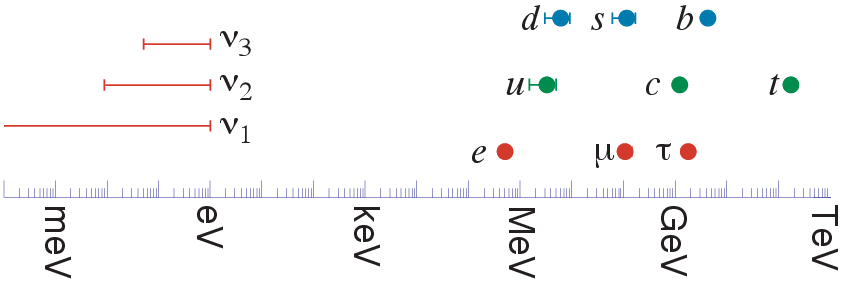
\includegraphics[width=0.85\linewidth]{ch1/figs/n_mass_comp.png}
\vspace{0.3cm}
\caption{Comparison of the masses of fermions in the Standard Model. Neutrino masses are six orders of magnitude lower than other fermions in Standard Model. Neutrino masses were estimated assuming the normal mass hierarchy and a loose upper bound \cite{Hewett:2012ns}.}
\label{n_mass_comp}
\end{figure}

\section{Weak interactions}
The weak interaction is one of the four fundamental forces described in the Standard Model. It has a short effective range and is responsible for the radioactive decay of nuclei. In the weak interaction, fermions can exchange three types of force carriers: W$^+$, W$^-$, and Z bosons. The interactions associated with the charged W$^+$ and W$^-$ bosons are known as charged current interactions, whereas those associated with the neutral Z boson are known as neutral current interactions. Together, these vertices form the basis for weak interactions between leptons in the Standard Model. The weak interaction does not preserve parity symmetry. \cite{wu_experiment}

During a weak decay, different final-state particles are produced depending on the charge and mechanism of the exchanged W boson. This can be understood by considering two types of beta decay illustrated by the Feynman diagram \ref{beta_decay_types}. A beta-minus decay with no initial charge converts a neutron into a proton at the same vertex. Thus, the interacting boson has to carry a negative charge and produces an electron at that vertex. Similarly, in a beta-plus decay, the boson is $W^+$ and thus a positron is formed. Neutrinos are created on the basis of an intermediate boson that carries the interaction. Thus, there are three neutrino flavors based on the three charged leptons (electrons, muons, and tau) and their corresponding antineutrinos. 

\begin{figure}[!htbp]
    \centering
    \vspace{0.5cm}
    % Beta-minus decay diagram (left side)
    \begin{minipage}{0.49\textwidth}
        \centering
        \begin{fmffile}{beta_decay}
            \begin{fmfgraph*}(150,150)
                % Define external vertices for Beta-minus decay
                \fmfleft{n}
                \fmfright{p,e,nu}

                % Internal interaction vertex
                \fmf{fermion}{n,v1}
                \fmf{fermion}{v1,p}
                \fmf{boson,label=$W^-$}{v1,v2}
                \fmf{fermion,tension=1.5}{nu,v2}  % Antineutrino arrow (points inward)
                \fmf{fermion,tension=1.5}{v2,e}   % Lengthened electron arrow

                % Labels
                \fmflabel{$n$}{n}
                \fmflabel{$p$}{p}
                \fmflabel{$e^-$}{e}
                \fmflabel{$\bar{\nu}_e$}{nu}

                % Dots on interaction vertices
                \fmfdot{v1,v2}
            \end{fmfgraph*}
        \end{fmffile}
    \end{minipage}
    \hfill
    % Beta-plus decay diagram (right side)
    \begin{minipage}{0.49\textwidth}
        \centering
        \begin{fmffile}{beta_plus_decay}
            \begin{fmfgraph*}(150,150)
                % Define external vertices for Beta-plus decay
                \fmfleft{p}
                \fmfright{n,e,nu}

                % Internal interaction vertex
                \fmf{fermion}{p,v1}
                \fmf{fermion}{v1,n}
                \fmf{boson,label=$W^+$}{v1,v2}
                \fmf{fermion,tension=1.5}{v2,nu}  % Neutrino arrow
                \fmf{fermion,tension=1.5}{e,v2} 

                % Labels
                \fmflabel{$p$}{p}
                \fmflabel{$n$}{n}
                \fmflabel{$e^+$}{e}
                \fmflabel{$\nu_e$}{nu}

                % Dots on interaction vertices
                \fmfdot{v1,v2}
            \end{fmfgraph*}
        \end{fmffile}
    \end{minipage}
    \vspace{0.5cm}
    \caption{Feynman diagrams illustrating the two types of beta decay. Left: Beta-minus decay, where a neutron decays into a proton, emitting an electron and an electron antineutrino via a virtual \(W^-\) boson. Right: Beta-plus decay, where a proton converts into a neutron, emitting a positron and an electron neutrino via a virtual \(W^+\) boson.}    \label{beta_decay_types}

\end{figure}


In particle physics, the Lepton number is the net number of leptons in a reaction. Particles are given a unit positive lepton number and antiparticles a unit negative number. Two emergent properties from the Standard Model of Physics are that the lepton flavor and total lepton number \( L \) are conserved quantities. Conservation of the lepton number has no theoretical motivation and is not associated with any gauge symmetry. The discovery of neutrino oscillations provided the first evidence that lepton flavor is not strictly conserved, suggesting there is physics beyond the Standard Model (BSM). Understanding the mechanism by which the neutrino gets its mass can provide additional evidence for physics beyond the Standard Model (BSM) physics. 

\section{Neutrino Mass}
\subsection{Dirac Mass Mechanism}
There is no mechanism in the Standard Model to give neutrino mass. One way to add mass would be to use four neutrino fields that couple via the Higgs mechanism. The Higgs mechanism requires the existence of a right-handed neutrino field because, in the Standard Model, interaction with the Higgs boson couples opposite-chirality fields. The weak interaction is parity violating, and thus only the left-handed neutrino and right-handed antineutrino are produced or observed via weak interactions. They alone cannot couple to the Higgs field. It is possible that the right-handed neutrino and left-handed antineutrino are sterile to weak interaction, such that they do not couple to W or Z bosons. However, this would not explain the relatively low observed neutrino mass limits. 

\subsection{Majorana Mass Mechanism}
A different approach is to consider neutrinos as Majorana fermions. Then the right-handed antineutrino, $\bar{\nu_R}$, could be coupled to the left-handed neutrino, $\nu_L$. Thus, the left-chiral field would correspond to the neutrino and the right-chiral field would correspond to the antineutrino, and the neutrino and antineutrino could only be distinguished by chirality. This mechanism was first postulated by the Italian physicist Ettore Majorana \cite{Majorana_1937}. Using the See-Saw mechanism, it could provide a basis for neutrino mass, and also explain why neutrinos are much lighter than any other Standard Model particles.

\subsection{See-Saw Mechanism}
The See-Saw mechanism attempts to explain the relatively low observed neutrino mass limits by including both Dirac and Majorana masses in the Lagrangian. This suggests that there would be two light neutrino and two heavy neutrino terms such that the Lagrangian is given by:

% and the Majorana term will have the form of:
% \begin{equation}\label{majorana_mass_terms}
% -\frac{1}{2}m^L_M(\bar{\nu}_L\nu_L^c+\bar{\nu}_L^c\nu_L)-\frac{1}{2}m^R_M(\bar{\nu}_R\nu_R^c+\bar{\nu}_R^c\nu_R)
% \end{equation}

% Using the charge conjugation operator C, charge conjugation of the field can be expressed as:
% \begin{equation}\label{charge_conjugation1}
% \nu^C=C\nu=i\gamma^2\nu^*
% \end{equation}
% and
% \begin{equation}\label{charge_conjugation2}
% \bar{\nu}^C=\nu^TC=\nu^Ti\gamma^2
% \end{equation}

\begin{equation}\label{mass_lagrangian}
\mathcal{L}_{mass} = -\frac{1}{2}(\bar{\nu}_L\bar{\nu}_R^c) \begin{bmatrix} m_M^L & m_D \\ m_D & m_M^R \end{bmatrix} \begin{bmatrix} \nu_L^c \\ \nu_R \end{bmatrix} + hc
\end{equation}
\noindent
$m_D$ is the Dirac mass term, $m_M^L$ and $m_M^R$ are the left- and right-handed Majorana mass terms, and $hc$ is the Hermitian conjugate of the prior term. The left-handed Majorana mass term is forbidden by $SU (2)$ symmetry, so we let $m_M^L \rightarrow 0$. Diagonalizing the resulting matrix gives two effective fields: 

\begin{equation}\label{mass_lagrangian_reduced}
\mathcal{L}_{mass} = -\frac{1}{2}(\bar{\nu}_L\bar{N}) \begin{bmatrix} m_\nu & 0 \\ 0 & M_N \end{bmatrix} \begin{bmatrix} \nu \\ N \end{bmatrix} + hc
\end{equation}
\noindent
The resulting eigenvalues are $M_\nu \approx \frac{m^2_D}{m_R}$ and $M_N \approx m_R$. We have thus identified the mass eigenstates for neutrinos. If one of the mass terms increases, the other has to decrease, explaining the origin of the `See-Saw' nomenclature. This would explain the very small mass of observed neutrinos. The left-handed light neutrinos and right-handed light antineutrinos would be the ones observed in current experiments. The heavy right-handed neutrinos and left-handed antineutrinos would have a huge phase space, thus a shorter half-life, and would have decayed quickly in the early universe. Experiments measuring neutrino mass would give insight into this mechanism. 

\subsection{Measuring neutrino mass}
There are four ways to study the neutrino mass. The first is to use results from cosmology. The Lambda-CDM model-based spectral fit to the Planck data and other observations of large-scale structures in the universe can be used to measure the sum of the neutrino masses. The sum of masses is one of the model's free parameters, and the current limit implies a $\Sigma m_\nu<0.23$ meV \cite{Planck_2015fie}. However, this sum is model-dependent and relies on an extensive understanding of how the universe evolved. 

A model-independent approach is to measure the mass of a neutrino kinematically. This is done by studying the endpoint of a beta decay spectrum, which would have a slight variation in shape depending on the neutrino mass. The KATRIN collaboration is performing such a direct mass measurement by looking at the tritium $\beta$-decay spectrum and has achieved a sensitivity of $m_\beta < 0.45 \text{ eVc}^{-2}$ at a $90\%$ confidence level \cite{katrin2025}.


The third approach is to use neutrino oscillation experiments, though these can only set a lower limit on $\Sigma m_\nu$ or $m_\beta$. The mass eigenstates of neutrinos form a complete, orthonormal basis. Similarly, the three flavors $\nu_e$, $\nu_\mu$, and $\nu_\tau$ form yet another orthonormal basis. Experiments indicate that these two eigenbases are rotated relative to each other. The Pontecorvo–Maki–Nakagawa–Sakata matrix represents the unitary transformation between the two bases as shown \cite{Maki_1962mu}:

\begin{equation}\label{pmns_matrix}
\begin{bmatrix} \nu_e \\ \nu_\mu \\ \nu_\tau \end{bmatrix} = \begin{bmatrix} U_{e1} & U_{e2} & U_{e3}\\ U_{\mu 1} & U_{\mu 2} & U_{\mu 3} \\ U_{\tau 1} & U_{\tau 2} & U_{\tau 3} \end{bmatrix} \begin{bmatrix} \nu_1 \\ \nu_2 \\ \nu_3 \end{bmatrix}
\end{equation}

Eq. \ref{pmns_matrix} is often expressed using three mixing angles ($\theta_{1,2}$, $\theta_{2,3}$ and $\theta_{1,3}$) and three phase angles ($\delta_{CP}$, $\alpha_1$ and $\alpha_2$).

\begin{equation}\label{pmns_matrix_expanded}
U = \begin{bmatrix} 1 & 0 & 0\\ 0 & c_{23} & s_{23} \\ 0 & -s_{23} & c_{23} \end{bmatrix} \begin{bmatrix} c_{13} & 0 & s_{23}e^{-i\delta_{cp}}\\ 0 & 1 & 0 \\ -s_{23}e^{-i\delta_{cp}} & 0 & c_{13} \end{bmatrix} \begin{bmatrix} c_{12} & s_{12} & 0\\ -s_{12} & -c_{12} & 0 \\ 0 & 0 & 1 \end{bmatrix} \begin{bmatrix} 1 & 0 & 0\\ 0 & e^{i\frac{\alpha_1}{2}} & 0 \\ 0 & 0 & e^{i\frac{\alpha_2}{2}}\end{bmatrix}
\end{equation}

where $c_{ij}=\mathrm{cos}(\theta_{i,j})$ and $s_{ij}=\mathrm{sin}(\theta_{i,j})$. This gives the probability that a neutrino of flavor $\alpha$ oscillates to flavor $\beta$ as:

\begin{equation}\label{n_oscillation}
P_{\alpha\rightarrow\beta} = \left|\sum_i U^*_{\alpha i}U_{\beta i} e^{-i\frac{m_i^2L}{2E}}\right|^2
\end{equation}

It can be shown that Eq. \ref{n_oscillation} depends on $\Delta m^2_{i,j}=m^2_i-m^2_j$ and not on individual masses. Thus, neutrino oscillation experiments can determine the squared difference of the masses and their sign, but not the individual masses of different flavors of neutrinos. We know from experiments such as SNO that $m_2>m_1$, but no information is available about the sign of $\Delta m_{23}^2$. Thus, it is not known which neutrino is the heaviest, nor the values of each of the mass eigenstates. This problem is called the neutrino mass hierarchy problem. If the mass $m_3$ is heavier than the mass $m_2$, the hierarchy is called normal, but if it is lighter, it is said to be inverted, as shown in figure \ref{mass_hierarchies_fig}.

\begin{figure}[!htb]
\centering
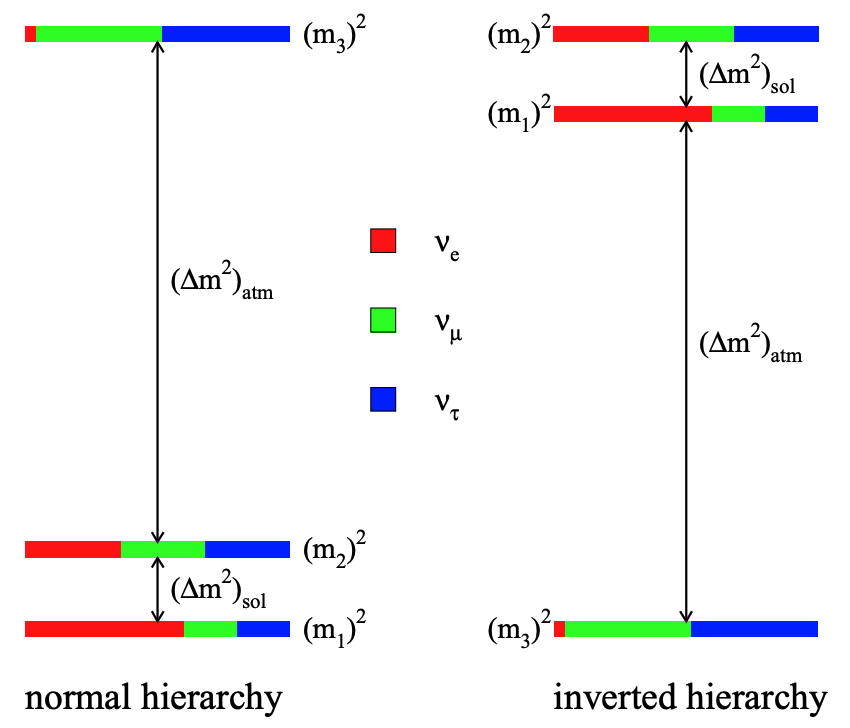
\includegraphics[width=0.75\linewidth]{ch1/figs/mass_hierarchies.png}
\caption{Two possible neutrino mass hierarchies. In the normal hierarchy (left), the lightest mass state is \( m_1 \), followed by \( m_2 \) (separated by the solar mass-squared difference \( \Delta m^2_{21} \)), with \( m_3 \) being the heaviest, separated by the atmospheric mass-squared difference \( \Delta m^2_{32} \). In the inverted hierarchy (right), \( m_3 \) is the lightest, while \( m_1 \) and \( m_2 \) are heavier. Figure from \cite{Hewett:2012ns}.}
\label{mass_hierarchies_fig}
\end{figure}

The fourth approach is to study double beta decay, which would probe the effective neutrino mass term $\langle m_{\beta\beta}\rangle$.

\section{Double Beta Decay}
Some nuclei need to undergo a beta decay to move close to the ideal ratio of protons to neutrons; however, they are energetically forbidden to undergo such a decay. Instead, these nuclei may undergo double beta decay to achieve the optimal ratio of nucleons. In double beta decay, two neutrons in the nucleus are converted to protons simultaneously, producing two electrons and two electron antineutrinos. It is represented by equation \ref{beta_decay_eq} and Feynman diagram \ref{ch1:fig:2nu2beta}. It was first discussed by M. Goeppert-Mayer, and there are 35 potential nuclei in nature that can undergo this process \cite{ZUBER_2012}.

\begin{equation}\label{beta_decay_eq}
(Z,A) \rightarrow (Z+2,A) + 2e^- + 2\bar{\nu}_e
\end{equation}

\begin{figure}[htbp]
  \centering
  \begin{fmffile}{2nu2beta_adjusted}
    \begin{fmfgraph*}(200,200)
      % Define left-side (incoming) and right-side (outgoing) vertices.
      \fmfleft{i1,i4}
      % Order the right vertices from top to bottom:
      % o1: top proton, o3: top electron, o5: top antineutrino,
      % o6: bottom antineutrino, o4: bottom electron, o2: bottom proton.
      \fmfright{o1,o3,o5,o6,o4,o2}
      
      % Hadronic lines: d -> u conversion.
      \fmf{fermion,tension=0.8}{i1,v1}
      \fmf{fermion,tension=0.5}{v1,o1}  % Top proton (u)
      \fmf{fermion,tension=0.8}{i4,v4}
      \fmf{fermion,tension=0.5}{v4,o2}  % Bottom proton (u)
      
      % W-boson propagators connecting quark vertices to lepton vertices.
      \fmf{photon,tension=0.65,label=$W^-$}{v1,v2}
      \fmf{photon,tension=0.65,label=$W^-$}{v4,v3}
      
      % Add a phantom edge to bring the leptonic vertices closer together.
      \fmf{phantom,tension=2}{v2,v3}
      
      % Leptonic lines:
      % From the top vertex (v2): electron and antineutrino.
      \fmf{fermion,tension=0.4}{v2,o3}  % Top electron (e)
      \fmf{fermion,tension=0.4}{v2,o5}  % Top antineutrino (\(\bar{\nu}\))
      % From the bottom vertex (v3): electron and antineutrino.
      \fmf{fermion,tension=0.4}{v3,o4}  % Bottom electron (e)
      \fmf{fermion,tension=0.4}{v3,o6}  % Bottom antineutrino (\(\bar{\nu}\))
      
      % Mark the internal vertices with dots.
      \fmfdot{v1,v2,v3,v4}
      
      % External labels:
      \fmflabel{$d$}{i1}          % Incoming down quark (from neutron)
      \fmflabel{$d$}{i4}          % Second incoming down quark
      \fmflabel{$u$}{o1}          % Top outgoing up quark (proton)
      \fmflabel{$u$}{o2}          % Bottom outgoing up quark (proton)
      \fmflabel{$e$}{o3}          % Top emitted electron
      \fmflabel{$e$}{o4}          % Bottom emitted electron
      \fmflabel{$\bar{\nu}$}{o5}   % Top antineutrino
      \fmflabel{$\bar{\nu}$}{o6}   % Bottom antineutrino
    \end{fmfgraph*}
  \end{fmffile}
  \vspace{0.5cm}
  \caption{Feynman Diagram for Two-Neutrino Double Beta Decay (2$\nu\beta\beta$) process.}
  \label{ch1:fig:2nu2beta}
\end{figure}


The necessary conditions for a double beta decay are shown in figure \ref{2nbb_cond}. Candida isotopes are neutron-rich, even-even nuclei that are forbidden to decay by beta decay but could decay via two simultaneous steps. Since such simultaneous decay of two nucleons in the same nucleus is very unlikely, double beta decay is a second-order weak process. It was first experimentally observed in $^{82}$ Se with a half-life of $(1.1^{+0.8}_{-0.3})\times 10^{20}$ years by Elliott, Hahn, and Moe. \cite{PhysRevLett.59.2020}. It has been observed in many more nuclei since then, such as $^{76}$Ge \cite{PhysRevLett.125.252502}, $^{136}$Xe \cite{PhysRevLett.107.212501}, $^{130}$Te \cite{Alduino2017}, etc.

\clearpage
\begin{figure}[!htb]
\centering
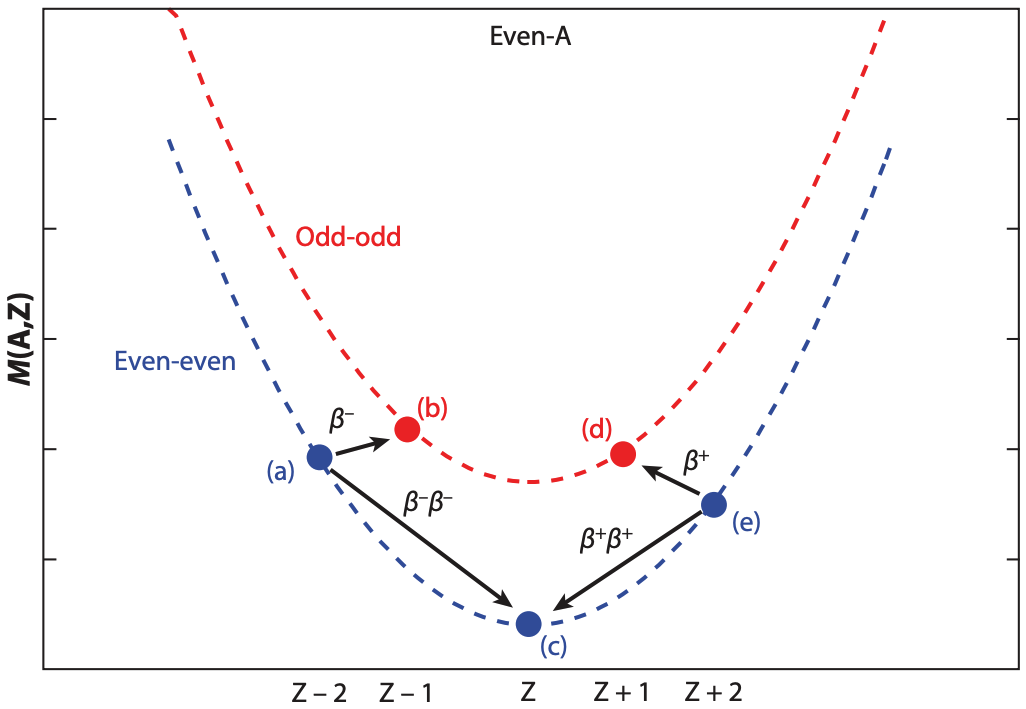
\includegraphics[width=0.85\linewidth]{ch1/figs/2nbb_cond.png}
\caption{Ground state mass parabola for nuclei showing the necessary conditions for double-beta decay. The plot shows nuclear charge \(Z\) versus nuclear mass \(M(A,Z)\). Double-beta decay is energetically allowed when the initial even-even nucleus has a higher mass than the final nucleus, and single beta decay is forbidden. Only even-even nuclei can undergo double-beta decay due to their greater stability. Figure from \cite{2nbb_cond}.}
\label{2nbb_cond}
\end{figure}

\section{Neutrinoless Double-Beta Decay}
If the neutrino were a Majorana particle, it would be possible to have a double beta decay without the emission of the two neutrinos. Instead, the neutrino would be exchanged as a virtual particle such that one nucleon absorbs the neutrino emitted by another. This process is called neutrinoless double-beta decay. This scenario, which is considered the simplest possible model, is termed ``light neutrino mediated'' decay. The general reaction would be as follows:

\begin{equation}\label{0nbeta_decay_eq}
(Z,A) \rightarrow (Z+2,A) + 2e^-
\end{equation}


\begin{figure}[!htb]
\vspace{0.5cm}
  \centering
  \begin{fmffile}{0nu2beta}
    \begin{fmfgraph*}(200,200)
      % External vertices:
      \fmfleft{i1,i4}        % Left: incoming quarks (from neutrons)
      \fmfright{o1,o2,o3,o4}   % Right: outgoing particles (protons & electrons)
      
      % Left-hand side fermion lines (d -> u conversion)
      \fmf{fermion,tension=0.8}{i1,v1}
      \fmf{fermion,tension=0.5}{v1,o1}   % u (proton) emerging top right
      \fmf{fermion,tension=0.8}{i4,v4}
      \fmf{fermion,tension=0.5}{v4,o4}   % u (proton) emerging bottom right
      
      % Leptonic lines (electrons) attached to intermediate vertices:
      \fmf{fermion,tension=0.4}{v2,o2}   % top electron
      \fmf{fermion,tension=0.4}{v3,o3}   % bottom electron
      
      % Dummy vertex for the Majorana mass insertion (no extra label)
      \fmf{plain,tension=1}{v5,v2}  % Removed arrow
      \fmf{plain,tension=1}{v5,v3}  % Removed arrow
      \fmfv{decor.shape=cross,decor.size=.1w}{v5}
      
      % W-boson propagators (labeled as W^-)
      \fmf{photon,tension=0.65,label=$W^-$}{v1,v2}
      \fmf{photon,tension=0.65,label=$W^-$}{v4,v3}
      
      % Mark the interaction vertices with dots
      \fmfdot{v1,v2,v3,v4}
      
      % External labels:
      \fmflabel{$d$}{i1}         % Incoming down quark (from a neutron)
      \fmflabel{$d$}{i4}         % Second incoming down quark
      \fmflabel{$u$}{o1}         % Outgoing up quark (proton)
      \fmflabel{$u$}{o4}         % Second outgoing up quark
      \fmflabel{$e$}{o2}         % Emitted electron (top)
      \fmflabel{$e$}{o3}         % Emitted electron (bottom)
    \end{fmfgraph*}
  \end{fmffile}
  \vspace{0.5cm}
  \caption{Feynman Diagram for light neutrino exchange neutrinoless double beta decay ({\onbb}) process.}
  \label{ch1:fig:0nu2beta}
\end{figure}

Figure \ref{ch1:fig:0nu2beta} shows the Feynman diagram for the process. An observable quantity of the process is the decay rate. Using Fermi's golden rule, it can be expressed as:
\begin{equation}\label{0nbbdecay_rate}
(T^{0\nu}_{1/2})^{-1} = G^{0\nu}\left|M_{0\nu}\right|^2\langle m_{\beta\beta}\rangle^2
\end{equation}
\noindent
The phase space term $G^{0\nu}$ corresponds to a phase space into which the electron can decay. The phase space can be calculated exactly for any given isotope. $M_{0\nu}$ is the nuclear matrix element (NME), also called the `transition amplitude'. It encapsulates all of the nuclear physics processes occurring inside the nucleus and can be understood as the probability of the transition between the initial and daughter nuclei. It is difficult to know the initial and final wave functions of the nuclei, so calculating nuclear matrix elements is non-trivial and is an active field of research \cite{Menendez:2017fdf}. Finally, $\langle m_{\beta\beta}\rangle$ is the effective neutrino mass term and can be represented as:

\begin{equation}\label{effective_mjd_mass}
\langle m_{\beta\beta}\rangle =  \left|\sum_{i=1}^{3} U^2_{ei}m_i\right|
\end{equation}
\noindent
$U_{ei}$ are the components of the PMNS neutrino mixing. This process described above assumes an exchange of a light Majorana neutrino, but there can be other exotic physics that can contribute to the decay rate (see \cite{Schechter_1982} for an example). However, all of these processes still imply that the neutrino is a Majorana particle.

Eq. \ref{0nbbdecay_rate} depends on the mass hierarchy and can help to probe the absolute neutrino mass scale. The observed decay rate would be different depending on the neutrino mass hierarchy. Figure \ref{majorana_mass} shows the range of $m_{\beta\beta}$ as a function of the lightest neutrino mass $m_l$ for the normal ordering and inverted ordering scenarios. If the neutrino masses are large compared to the size of the mass splittings, we do not expect a significant effect on $m_{\beta\beta}$, as both hierarchies merge at higher masses; however, if the neutrino masses are similar in magnitude to the mass splittings, there would be a difference in $m_{\beta\beta}$ based on the hierarchy. {\onbb} studies provide a fourth and unique way to understand neutrino mass, as they probe the effective Majorana mass $\langle m_{\beta\beta}\rangle$ and provide a direct way to measure the ordering of neutrino mass. However, detecting this extremely rare process requires meticulous background reduction and large-mass experiments.

\begin{figure}[!htb]
\centering
%[trim={left bottom right top},clip]
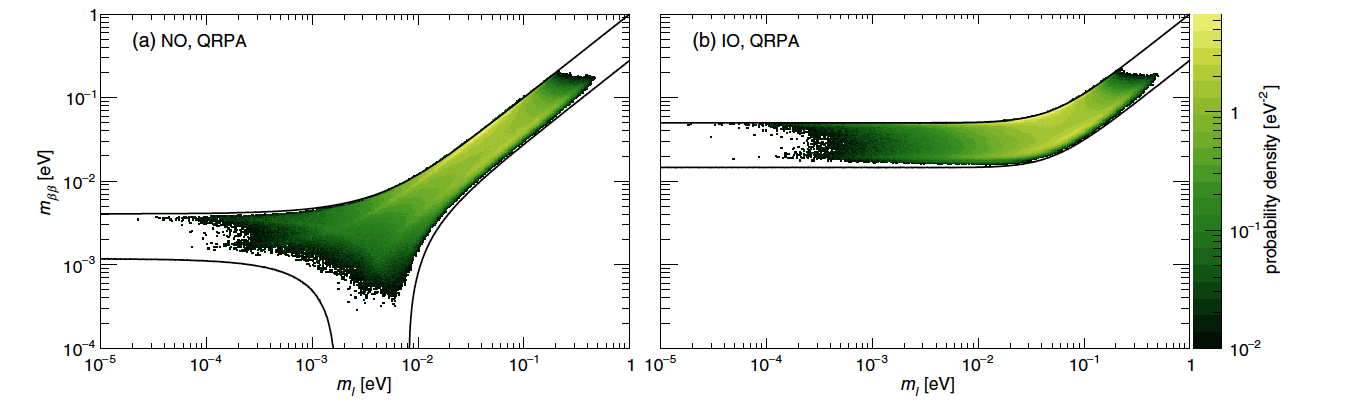
\includegraphics[trim={0.6cm 0cm 1cm 0cm},clip,width=\linewidth]
{ch1/figs/benato_posterior.png}
\caption{Parameter space for $m_{\beta\beta}$ and $m_l$ for the normal (right) and inverted (left) mass ordering. The allowed parameter space assuming $3\sigma$ intervals of the neutrino oscillation observables from NuFIT is shown by the solid solid lines \cite{nufit}. The marginalized posterior distributions for $m_{\beta\beta}$ and $m_l$ is shown by the color bar. This was obtained by combing equation \ref{effective_mjd_mass} with neutrino oscillation measurements. Plot assumes QRPA NMEs and the absence of mechanisms that drive $m_{\beta\beta}$ and $m_l$ to zero. Source: \cite{PhysRevD.96.053001}}
\label{majorana_mass}
\end{figure}


\section{Detecting Neutrinoless Double Beta Decay}
Numerous experiments have searched for neutrinoless double-beta decay ($0\nu\beta\beta$), and many are currently searching for it. The observable of interest is the sum of the kinetic energies of the two emitted electrons. If no antineutrino is emitted, the emitted electrons should carry the full energy difference between the final and initial nuclear states (the Q-value of the reaction). The experimental signature of such a decay would be a monoenergetic peak in energy at the end point of the two-neutrino spectrum, indicating that no antineutrinos are emitted, as shown in figure \ref{mjd_background_fig}. Most $0\nu\beta\beta$ experiments involve having a source of double-beta decay that acts as both a source and a detector. The region of interest (ROI) is defined as the narrow energy window around $Q_{\beta\beta}$ and is selected according to the energy resolution of the detector. Using radioactive decay theory, the number $0\nu\beta\beta$ of candidate events observed in the ROI is given by: %\cite{annurev_nucl}

\begin{equation}\label{roi_candidate}
N=\ln(2)\frac{N_A}{W}\left(\frac{a\epsilon MT}{T^{0\nu}_{1/2}}\right)
\end{equation}
where $N_A$ is Avogadro's number, $W$ is the molar mass of the source, $a$ is the isotopic abundance of the parent isotope, $\epsilon$ is the detector efficiency of the signal in the ROI, and $t$ is the observed time. Using Eq. \ref{roi_candidate}, we can understand how the half-life sensitivity depends on the detector:

\begin{equation}\label{det_sensitivity}
T^{0\nu}_{1/2} \propto
    \begin{cases}
    aM\epsilon T & \text{(background free)}\\
    a\epsilon\sqrt{\frac{MT}{B\Delta E}} & \text{(with background)}
    \end{cases}       
\end{equation}
such that $\Delta E$ is the energy resolution of the detector, and B is the background index of the experiment normalized to the width of the ROI, source mass, and measurement time. The importance of low background is apparent as $T^{0\nu}_{1/2}$ scales linearly with run time t for a no background experiment compared to $\sqrt{t}$ in the presence of backgrounds.


\begin{figure}[!htb]
\centering
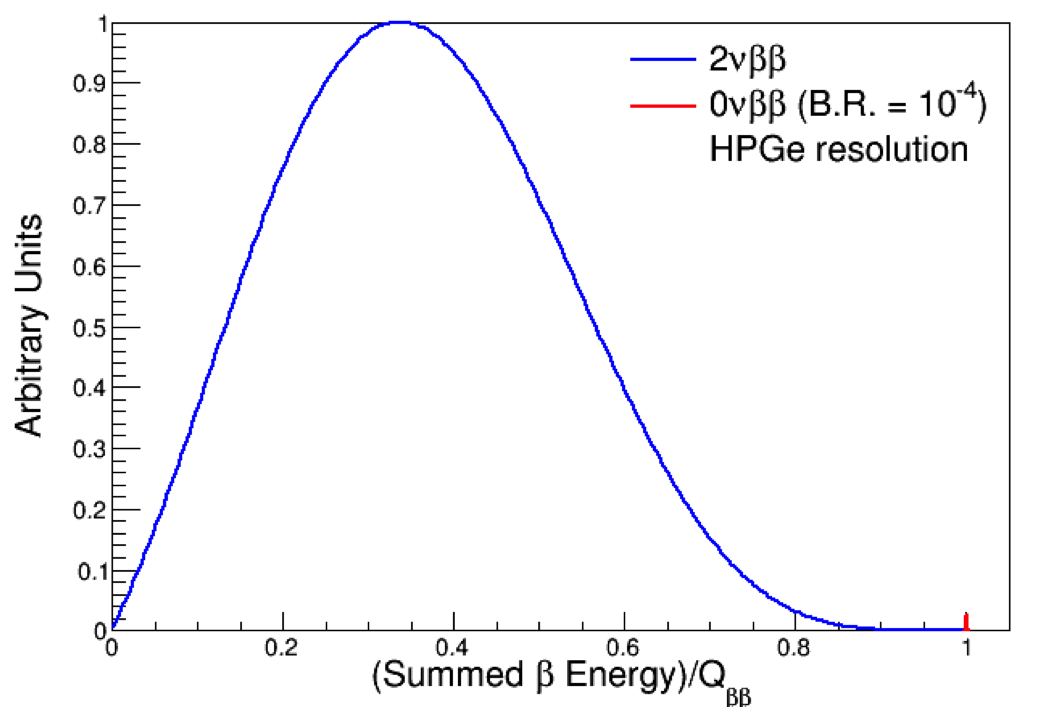
\includegraphics[width=0.9\linewidth]{ch1/figs/DoubleBetaEnergy.png}
\caption{Simulated $0\nu\beta\beta$ signal in a ${}^{76}\mathrm{Ge}$ detector. The {\onbb} signal is shown with an assumed half life of $10^{25}$ \cite{mjd_background} years.}
\label{mjd_background_fig}
\end{figure}

For a substantial probability of discovery, experiments that seek $0\nu\beta\beta$ need to have a source as large as possible with extremely low backgrounds. At that sensitivity level, natural isotopes such as $^{222}$Rn, $^{232}$Th, and $^{232}$U can introduce background events. Cosmic rays are another potential source, along with the decay of {\tnbb} depending on the energy resolution of the experiment. Most of the experiments are thus housed underground to decrease the rate of cosmic-ray-induced backgrounds and cosmogenic activation of detector materials. They are also heavily shielded, and the experimental parts are ultra-clean. The experimental programs also need to perform radioactive assay studies to understand the backgrounds of their experiments.

\begin{figure}[!htb]
\centering
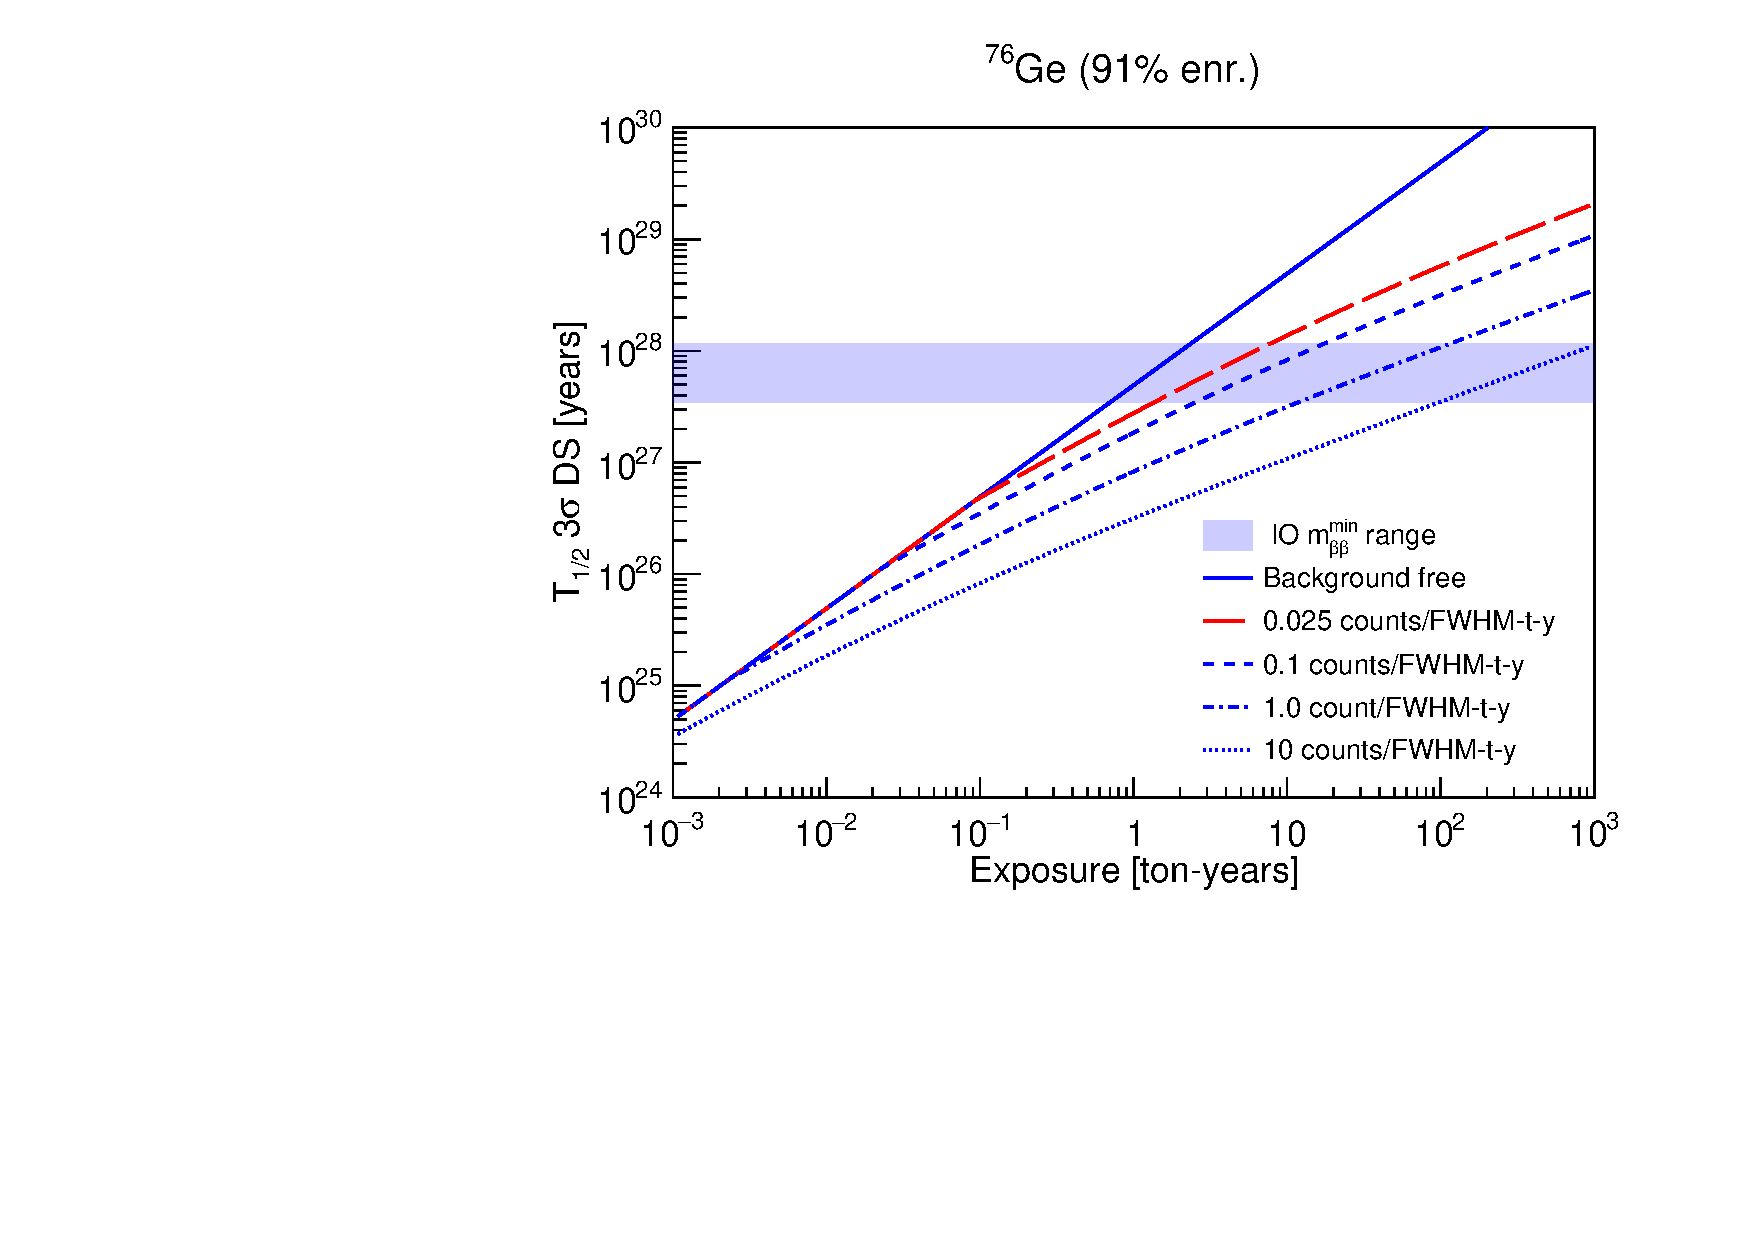
\includegraphics[width=0.99\linewidth]{ch1/figs/ThreeSigDL.pdf}
\caption{The exposure needed for 3$\sigma$ confidence level discovery of neutrinoless double beta decay for different half life limit, given the inverted hierarchy. Various lines represent scenarios with different background levels in ROI. Red line indicate the {\Lthou} background goal. The blue band shows the bottom of the inverted ordering.}
\label{exposure_plot}
\end{figure}

The $\beta\beta$ isotope used should ideally have a high Q value and a low double beta decay rate. It must also be able to turn into large detectors to increase the probability of discovery. Several isotopes are used in experiments searching for neutrinoless double beta decay, including ${}^{76}\mathrm{Ge}$ (GERDA \cite{GERDA_final}, {\MJD} \cite{Majorana_final}), ${}^{136}\mathrm{Xe}$ (KamLAND-Zen \cite{KamLAND-Zen:2024eml}, nEXO \cite{nEXO:2021ujk}), and ${}^{130}\mathrm{Te}$ (CUORE \cite{Arnaboldi2002du}, SNO $+$ \cite{SNO_paper}). KamLAND-Zen established the leading half-life limit in $^{136}$Xe with $T^{0\nu}_{1/2} > 2.23 \times 10^{26}$ years \cite{KamLAND-Zen:2024eml}. 


In the coming years, the next generation of experiments will attempt to explore the entire inverted hierarchy region of figure \ref{majorana_mass}. Figure \ref{exposure_plot} shows the exposure needed to achieve the discovery of $3\sigma$ at the bottom of the inverted hierarchy region in ${}^{76}\mathrm{Ge}$. The different lines represent background levels in counts per Region of Interest (ROI). The different background scenarios underscore the importance for experiments to reduce or eliminate all of their background in ROI and follow the solid blue line. As the experiments increase their exposure time, the sensitivity will increase and reach the bottom of the inverted hierarchy band. The bottom of the band is shown with the shaded blue box, which is calculated by using various calculations of nuclear matrix elements. Next-generation experiments would test an inverted hierarchy space and provide new insight into the nature of neutrinos.

Thus, the next decade would be an exciting time for research in neutrino physics. With ton-scale experiments such as {\Lthou} \cite{legend2017}, there might be major revelations about the properties of the neutrino. We might find that neutrinos are their antiparticles, or at least that inverted ordering is not true. In that case, new experiments and possible theories must be postulated to explain the neutrino mass and its interaction. Neutrinoless double beta decay will inform a new Standard Model of physics. In the next section, we explore ${}^{76}\mathrm{Ge}$ as a choice of detector and the LEGEND experiment's search for neutrinoless double-beta decay.